\chapter{Planification et demande}

\begin{center}
    \makebox[\textwidth]{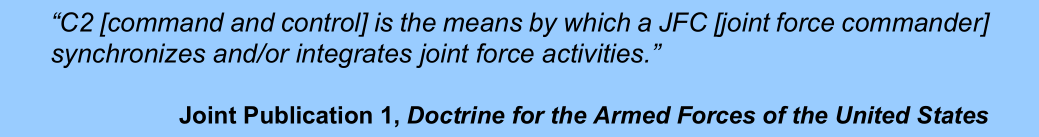
\includegraphics[width=\paperwidth]{quote3.png}}
\end{center}

\section{Introduction}

Ce chapitre décrit le processus de prise de décision \gls{cas}, décrit les responsabilités du staff, établit les bases de ce qu'il y a lieu de prendre en compte lors de la planification, et établit les procédures de requêtes de \gls{cas}.

La phase de planification commence lorsque l'unité reçoit l'ordre du Haut Commandement.

Bien que chapitre se concentre principalement sur les tâches à effectuer lors d'opération complexes, les même tâches peuvent s'appliquer aux opérations d'exfiltration, de \gls{csar}, qui pourraient avoir une structure de commandement différente.


\e
    \item Il existe deux types de \gls{cas} distincts:
    \ee
        \item Le \gls{cas} planifié
        \item Le \gls{cas} immédiat
    \ed
\ed

\section{Mission}

Le \gls{cas} est intégré au reste du dispositif de la coalition en opérations défensives et offensives, pour détruire, neutraliser, interdire, retarder ou empêcher le mouvement de l'ennemi.
\e
	\item Le \gls{cas} peut servir pour renforcer les opérations annexes, soutenir l'effort majeur ou établir les zones de sécurité
	\ee
		\itemt{Opérations annexes}{
		Bien que ce ne soit pas vocation principale, le \gls{cas} peut être employé pour soutenir une opération loin en territoire ennemie (infiltration, exfiltration, opérations spéciales), ou pour une opération ponctuelle}
		\itemt{Opérations de combat rapproché}{
		Le plus souvent, le \gls{cas} servira à renforcer l'effort de guerre principal. Les appareils de \gls{cas} ajoutent leur force aux forces au sol pour soutenir les \glspl{gc}. La vitesse et la portée du \gls{cas} en font un élément idéal pour exploiter les avancées amies, contrer les manoeuvres adverses ou poursuivre un ennemi en fuite.}
		\itemt{Opérations de sécurité}{
		Le \gls{cas} est efficace pour empêcher la pénétration de l'ennemi. Le temps de réponse et la puissance de feu du \gls{cas} peut augmenter de beaucoup la force des unités au sol.}
	\ed
	\item Le \gls{cas} peut servir pour les opérations offensives, défensives et de stabilité
	\ee
		\itemt{Le \gls{cas} en support de l'offense}{
		\eee
			\itemt{Mouvement vers le contact}{
			Le \gls{cas} peut servir à appuyer les forces au sol qui font mouvement. Une fois le contact avec l'ennemi établi, le \gls{cas} peut les submerger et accélérer le déploiement des forces alliées. \textbf{Pendant la planification de l'intégration du \gls{cas} à l'avancée alliée, il est recommandé de déployer les appareils tout le long de l'axe de progression.}}
			\itemt{Attaque}{
			Les \gls{gc} peuvent utilser le \gls{cas} pour attaquer directement l'ennemi. Le \gls{cas} peut détruire les unités ou capacités ennemies importantes avant que l'ennemi ne puisse établir de défense. Le \gls{cas} peut également servir à renforcer la puissance de feu lors d'une attaque, ou pour isoler une force ennemie sur le champ de bataille et la forcer à prendre une position défensive.}
			\itemt{Exploitation}{
			L'exploitation est une tactique offensive utilisée après une attaque réussie, et sert à déstabiliser l'ennemi, en coupant les voies d'accès, en détruisant les forces qui font retraite, et pour frapper les cibles d'opportunité lorsque la cohésion de l'ennemi diminue.}				\itemt{Poursuite}{
			En poursuite, le \gls{gc} attaque l'efficacité de l'ennemi en fuite alors qu'il est démoralisé et que sa cohésion et sont contrôle sont faibles. Puisque l'objectif de la poursuite est la destruction de l'ennemi, le \gls{cas} peut maintenir une pression directe et constante sur l'ennemi pour empêcher qu'il ne se réorganise ou ne se reconstitue.}
		\ed}
		\item Le \gls{cas} en support des opérations défensives alliées
		\eee
			\itemt{Support de la manoeuvre}{
			Le \gls{cas} peut s'ajouter à la puissance de feu des unités au sol en tant que membre d'une force combinée}
			\itemt{Support du mouvement}{
			Le \gls{cas} peut soutenir les éléments alliés lors de leurs mouvements entre deux positions. Les \gls{gc} peuvent utiliser le \gls{cas} pour protéger le front, les flancs ou l'arrière de la formation en mouvement.}
			\itemt{Refoulement de l'ennemi}{
			Le \gls{cas} peut servir à refouler une force ennemie qui aurait franchi ou pénétré les défenses alliées}
		\ed
		\itemt{Le \gls{cas} en opération de stabilité}{
		L'emploi du \gls{cas} en opération de stabilité est foncièrement différent de l'emploi du \gls{cas} en opération de combat. Comme l'objectif d'une opération de stabilité est d'établir la sécurité civile, rétablir les services, et restaurer et protéger les infrastructures, le \gls{cas} en opération de stabilité sera généralement restreint en terme d'échelle et des \glspl{roe} strictes seront souvent d'application. L'utilisation de \glspl{pgm} sera souvent préconisé par le \gls{jfc} lors du support de \gls{gc} en environnement urbain, de manière à limiter les dommages collatéraux.
		}
	\ed
\ed

\section{Ennemi}

Lors de la planification, il faut tenir compte de la disposition des forces ennemies, leur composition, son \gls{aob}, et ses intentions probables.

\e
	\item Autres considération:
	\ee
		\item Quelles sont les capacités offensives et défensives de l'ennemi?
		\item Quelles sont les capacités ennemies concernant:
		\eee
			\item Menaces sol-air
			\item Leurres
			\item Camouflage
		\ed
		Les cibles de hautes importance seront généralement défendue par des unités anti-aériennes. L'utilisation d'armes à très longue portée et le fait de varier les \glspl{ip} augmentera les chances de survies des appareils de \gls{cas}.
		\item Quelles sont les capacités de l'ennemi en terme d'\gls{ew} ou de \gls{cc}?
	\ed
	\item A partir de ces informations, le planificateur peut anticiper les capacités de l'ennemi à contrer la mission alliée, et l'influence potentielle qu'aura l'ennemi sur les vols alliés. Les changements susceptibles de se produire pendant le déroulement de la mission rendent les communications avec les appareils en vol très importantes, nécessitant parfois une adaptation du plan de vol, c'est pourquoi des alternatives sont prévues dès le commencement de la mission.
\ed

\section{Troupes au sol alliées}

Le planificateur doit prendre en compte les unités \gls{cc}, \gls{isr}, \gls{ew} et \gls{cas}.

\e
	\itemt{Unités \gls{cc}}{
	Un plan \gls{cc} détaillé, flexible et redondant est essentiel. Des unités \gls{cc} aéroportées peuvent faciliter le travail du \gls{cc}, mais chaque plateforme a ses capacités et limitations qui doivent être prises en compte lors du planning. Au minimum, les points suivants doivent être évalués:}
	\ee
		\itemt{Unités \gls{cc} aéroportées}{
		Est-ce que ces unités ont une importance critique pour la mission ou seulement pour une partie de celle-ci? Quel sont le rôle et la fonction de chacune? Est-ce que le nécessaire a été fait pour assurer la communication entre le \gls{cc} et les \gls{rw} volant bas?}
		\itemt{Unités Gls{cc} au sol}{
		Intégrer les unités \gls{cc} au sol revêt une importance capitale. Quel sont le rôle et la fonction de chacune? Est-ce que le nécessaire a été fait pour assurer les communications avec le \gls{cc}?.}
	\ed
	\itemt{Unités \gls{isr}}{
	Toutes les sources d'\gls{isr} sont d'excellentes (drone, \gls{elint}, scouts, \gls{faca}, rapports des appareils d'attaque, etc.) sources d'informations.}
	\itemt{Capacités et armement des appareils \gls{cas}}{
	Le planificateur choisit les combinaisons d'appareils et d'armement qui offrent la précision, la puissance et la flexibilité nécessaires pour obtenir l'effet désiré. Le \gls{gc} doit fournir suffisamment d'informations à propos de cet effet désiré, ainsi que toute restriction tactique ou limitation. Les \gls{gc} doivent savoir qu'une requête de \gls{cas} immédiate risque d'être assurée par un appareil ne disposant pas de l'armement optimal pour la mission.}
\ed

\section{Terrain}

\e
	\itemt{Comment le terrain affecte le \gls{cas}}{
	Le terrain peut affecter les communications et la \gls{los}. Les unités \glspl{rw} sont particulièrement concernées. Le planificateur doit compenser ces limitations en implémentant des relais, ou intégrer ces limitations à la mission. La visibilité et le plafond peuvent affecter la décision d'employer des tactiques basse, moyenne ou haute altitude, ou l'utilisation de \glspl{rw}. Ces conditions affectent également la capacité du \gls{jtac} à voir la cible. Si des véhicules ennemis se déplacent, une colonne de fumée peut révéler leur emplacement. La visibilité a un impact plus important sur les armes à longue portée (bombe lisse, roquettes) que sur les armes à courte portée (canon, bombes freinées). Un brouillard épais a plus d'impact sur les attaques à bas niveau. Une visibilité réduite et une couche nuageuse importante peuvent restreindre l'emploi de l'armement \gls{eo}. L'acquisition de la cible est généralement plus facile lorsque le soleil se trouve derrière l'appareil qui attaque.}
	\ee
		\itemt{Masquage de la cible}{
		Une cible masquée par le terrain, un immeuble ou une couverture naturelle peut être difficile à repérer. Une altitude plus élevée peut aider.}
		\itemt{Imagerie thermique}{
		Un grand nombre de variables affecte l'efficacité de l'imagerie thermique. L'état de l'équipement, l'heure de la journée et l'arrière-plan doivent être pris en compte.}
		\itemt{Contraste et luminosité}{
		Le contraste de la cible avec son arrière plan est un facteur critique lors de la recherche de cible. Une cible camouflée devant un arrière-plan de couleur similaire peut être impossible à détecter depuis une haute altitude ou une grande distance. Toutes les cibles, quelque soit le contraste, sont plus difficiles à repérer en condition de faible luminosité.}
		\itemt{Environnement montagneux}{
		Un environnement montagneux peut forcer l'ennemi à concentrer ses forces sur les routes, dans les vallées, sur des pentes plus faibles ou dans de profond défilés, là ou le \gls{cas} est très efficace. Cependant, ce type de terrain restreint également la direction d'attaque des appareils \gls{cas}. Le planificateur doit supposer que l'ennemi va concentrer ses défenses sur l'axe d'attaque le plus probable.}
		\itemt{Environnement désertique}{
		Les appareils \gls{cas} sont rendus plus vulnérables par l'absence de couverture, et la dispersion des unités au sol.}
		\eee
			\itemt{Acquisition de la cible}{
			En général, comme le contraste entre la cible et l'arrière plan est fort, la détection sera possible à plus longue portée.}
			\itemt{Emploi des armes}{
			Un environnement désertique permettra généralement l'emploi des armes à leur portée maximale.}
			\itemt{Communications}{
			En environnement désertique, les communications sont généralement possible à plus longue portée.}
			\itemt{Menaces}{
			Les menaces seront également capables d'acquérir et d'engager les appareils \gls{cas} à portée maximale.}
			\itemt{Manque de références}{
			Le désert, de par l'absence de références distinctes au sol, rend le talk-on et l'établissement d'\gls{ip} difficiles}
		\ed
		\itemt{Jungle/forêt}{
		Généralement, le contact avec l'ennemi se fera à très courte portée.}
		\eee
			\itemt{Acquisition de la cible}{
			L'acquisition de la cible peut être rendue difficile, voire impossible, par la densité des arbres, pour l'appareil qui attaque comme pour le \gls{jtac}. Dans ces conditions, il appartient au \gls{gc} de marquer la cible. Un \gls{faca} en station peut également aider de par sa \gls{sa} supérieure.}
		\ed
		\itemt{Environnement urbain}{
		Le \gls{cas} en environnement présente des particularités uniques, parmi lesquelles la déconfliction en espace confiné, des \glspl{roe} particulières, la difficulté d'analyser la menace, la présence de non-combattants, le risque de dégâts collatéraux et l'augmentation du risque de tir fratricide.}
		\eee
			\itemt{Menaces}{
			La ville offre d'excellent couvertures aux unités anti-aériennes. Les \glspl{sam} ou \gls{aaa} légers peuvent être employés depuis les toits. Le terrain encombré peut rendre l'acquisition des menaces difficile. Le placement des zones d'attente est rendu difficile par la dispersion des menaces dans une grande zone urbaine. Les \glspl{rw} nécessitent un secteur sécurisé de manière à pouvoir se déplacer est être moins prévisibles. Les \glspl{fw} établissent leur zone d'attente en terrain non-hostile, mais suffisamment proche de la ville que pour pouvoir assurer un support rapide.}
			\eeee
				\item Infrarouge et \glspl{nvg}
				\eeeee
					\item Les signatures infrarouges sont affectées par la proximité des bâtiments. La température généralement plus haute en environnement urbain affectent négativement le contraste infrarouge entre la cible et l'arrière-plan.
					\item Les lumières de la ville peuvent saturer les \glspl{nvg} et les rendre inutiles.
				\ed
				\itemt{\gls{cc}}{
				L'environnement urbain présente de gros problèmes de communications du fait des immeubles qui bloquent la \gls{los} et absorbent ou reflètent les signaux. L'utilisation d'un \gls{cc} aéroporté ou de relais permet d'en minimiser l'impact.}
				\itemt{Particularités propres au \gls{jtac}}{
				Les hauts bâtiments rendent l'acquisition de la cible par le pilote difficile, et peuvent nécessiter l'emploi de \gls{fah} spécifiques. Des observateurs peuvent être placés sur les toits pour améliorer la vue d'ensemble.}
				\itemt{Efficacité}{
				Un entraînement spécifique à l'environnement urbain est nécessaire pour que le \gls{jtac} y soit efficace. Historiquement, les engagements en zone urbaine se produisent dans 90\% des cas lorsque les troupes amies se trouvent à moins de 50 mètres des forces ennemies, et 80\% des blessures en zone urbaine proviennent des débris de verre dûs aux ondes de choc et aux surpression faisant suite à une explosion. Le \gls{jtac} doit porter une attention particulière à sélectionner l'armement approprié. La situation en zone urbaine change très rapidement, de bâtiment en bâtiment. Le \gls{jtac} peut utiliser les appareils de \gls{cas} ou le \gls{faca} pour engager des forces ennemies en dehors de la zone d'engagement, pour empêcher ces dernières de renforcer la ligne de front.}
				\itemt{Navigation}{
				La navigation est plus difficile en ville. Les bâtiments ne sont pas indiqués sur les cartes. Les mouvements rapides peuvent embrouiller les observateurs au sol ou en l'air concernant les positions amies et ennemies.}
				\itemt{\gls{grg}/Grille urbaine}{
				Des cartes ou des images détaillée de la zone urbaine peuvent être établies. Ces cartes ou ces images représentent la zone urbaine et peuvent contenir des bâtiments numérotés, les zones d'atterrissage pour les \glspl{rw}, des points de références, etc. C'est la responsabilité du \gls{gc} d'établir les cartes/images pour sa zone, et d'en assurer la gestion des versions ainsi que la diffusion. \textbf{Ces grilles doivent être établies en prenant en compte ce que les appareils de \gls{cas} pourront repérer le plus facilement (rivières, carrefours, bâtiments remarquables, ponts, etc.)}. Recommandations pour la création de \gls{grg}:}
				\eeeee
					\item L'image doit contenir une flèche pointant vers le nord, et être idéalement orientée avec le haut vers le nord
					\item Les coordonnées est et nord doivent se trouver en haut et à gauche
					\item Les bâtiments doivent être numérotés du nord-ouest au sud-est pour de grandes zones, ou dans le sens des aiguilles d'une montre à partir de l'objectif pour de plus petites zones
				\ed
			%\ed
			\efig{urbangrid}{Grille urbaine}
			%\re
				\item test
			\ed
			% Resume p88
		\ed
	\ed
\ed

\section{Le CAS planifié}

\e
    \item Le ``\gls{cas} request'' est effectué par l'unité qui demande un soutien aérien. On distingue deux principaux types de demandes:
    \ee
        \item Le \gls{cas} planifié à l'avance (``pre-planned \gls{cas}'', ou simplement ``\gls{cas}'')
        \item Le \gls{cas} ``à la demande'' (``on-call cas''), qui regroupe deux possiblités:
        \eee
            \item Le \gls{xcas}, où l'appareil en attente de tasking se trouve déjà dans les airs
            \item Le \gls{gcas}, où l'appareil en attente de tasking se trouve encore au sol
        \ed
    \ed
    \item Un ``\gls{cas} request'' réel se compose d'un grand nombre d'informations, utiles à la planification de la mission et à la répartition des effectifs disponibles.
    \item
    Souvent, pour DCS, l'équivalent du ``\gls{cas} request'' sera contenu dans le briefing de la mission (zone d'opération, menace, composition et force de unités ennemies, timing, emport, unités amies, \gls{jtac}, plan de fréquences, etc…).
    \item Toute référence ultérieure au ``\gls{cas} request'' fera donc implicitement référence au briefing de mission.
    \item Les considération à prendre en compte lors de l'établissement d'une \gls{cas} request sont propres au rôle de \gls{gc}/\gls{jfc} et ne seront pas traitées dans ce document.
    \item Le \gls{cas} planifié est un \gls{cas} effectué après une requête spécifique, concernant une zone connue, pour atteindre un objectif déterminé.
    \item Dans le cas d'un \gls{cas} planifié, un grand nombre de paramètres sont connus avant le décollage, ce qui permet une meilleure préparation.
\ed

\subsection{Étape 1: réception de l'ordre de mission}

\e
    \item
    En tant que participants au processus de planification, les officiers en charge (chef de patrouille, commandant d'escadron, …) devraient être à même de comprendre et analyser l'information à partir de ces différentes sources:
    \ee
        \item \gls{aob}
        \item \gls{ato}
        \item \gls{aco}
        \item \gls{spins}
        \item \gls{opord}
        \item \gls{sop}
    \ed
\ed
\note{Les \glspl{sop} sont propres à l'escadron, et sont normalement connues par les tous les officiers supérieurs.
    
    Exceptés les \glspl{sop}, tous les éléments sont normalement fournis sous une forme ou l'autre dans le briefing de mission.
    
    S'il devait manquer un élément, il appartient à l'officier en charge de la patrouille d'évaluer son importance et de poser les questions nécessaires à l'organisateur de la mission.
}

\subsection{Étape 2: analyse de la mission} 

\e
    \item Avant de pouvoir préparer la mission, les officiers en charges devront:
    \ee
        \item Mettre à jour les différentes sources d'informations (\gls{ato}, \gls{spins}, \gls{aco}, …)
        \item Estimer les capacités des forces à leur disposition (équipement, personnel, restrictions, …)
        \item Déterminer les tâches essentielles de la mission
        \item Évaluer les conditions relatives à:
        \eee
            \item L'ennemi
            \item La météo
            \item Le terrain
        \ed
        \item Avertir les unités (personnes) subordonnées
    \ed
    \item Considérations clefs à prendre en compte lors de l'analyse de la mission:
    \ee
        \item \gls{conops}: Quelles sont les intentions du \gls{jfc}? Attaque ou de défense? Surprise ou délibéré? Règles d'engagement?
        \item Comment s'intègre le \gls{cas} au reste du dispositif?
        \item Quelles pourraient être les intentions de l'ennemi? Comment ces intentions sont-elles affectées par le terrain, la météo, l'heure ?
        \item Quels sont les moyens de surveillance ou de reconnaissance à notre disposition?
        \item \gls{complan} Comment vont s'organiser les communications? Est-ce que toutes les unités participantes au \gls{cas} sont intégrées au \gls{complan}  de manière fiable et redondante?
    \ed
    \item Dans le cas d'une demande de \gls{cas} pré-planifié, un grand nombre d'informations supplémentaires pourront être obtenues via la demande elle-même. Par exemple:
    \ee
        \item Zone de \gls{cas}
        \item Menaces
        \item Type de cibles
        \item Localisation de la cible
        \item Localisation des forces amies
        \item Type de terrain
        \item Restrictions horaires
        \item \gls{jtac}
    \ed
\ed

\subsection{Étape 3: préparation de la mission}

\e
    \item Le ``Mission planning'', ou ``préparation de la mission'', est une étape cruciale au bon déroulement de cette dernière.
    \item Cette préparation sera effectuée par le chef de patrouille, qui sera chargé de rassembler et analyser toutes les informations à sa disposition pour préparer au mieux la mission de la patrouille dont il a la charge.
    \item Lorsque c'est possible, la préparation de la mission se fait en collaboration avec les différents éléments impliqués, certainement avec le \gls{jtac} en charge de la zone attribuée à la patrouille, le \gls{tacon}, et les autres chefs de patrouilles opérant dans le même théâtre opérationnel.
    \item Le chef de patrouille veillera tout particulièrement à toujours utiliser les informations les plus récentes, et fera attention à se tenir au courant de l'évolution de la situation.
    \item Il devra également s'assurer que tous les éléments sous son contrôle ont reçu et compris ses intentions pour la mission.
    \item Checklist de préparation de mission: \fullref{ann1}
\ed

\section{Le CAS immédiat}

\e
    \item Le \gls{cas} immédiat intervient lorsque la situation sur le champ de bataille évolue de manière inattendue.
    \item L'\gls{ato} peut allouer un certain effectif pour se préparer à répondre à ces situations.
    \item Le chef de patrouille trouvera alors dans cet \gls{ato} les informations nécessaires pour préparer son vol (emport, point d'attente, etc…).
    \item
    Pendant le vol (ou au parking pour le \gls{gcas}), si l'intervention de la patrouille s'avère nécessaire, celle-ci recevra un point de contact initial, ainsi que le call-sign et la fréquence de l'agence qui s'occupera de son contrôle terminal.
\ed





